\documentclass[a4paper,11pt]{article}
\usepackage[brazil]{babel}
\usepackage[utf8]{inputenc}
\usepackage{times}
\usepackage[T1]{fontenc}
\usepackage{amsmath,amssymb}
\usepackage{url}
\usepackage[square]{natbib}
\usepackage{indentfirst}
\usepackage{fancyhdr}
\usepackage{graphicx}
\usepackage{float}
\usepackage{booktabs,array}
\usepackage{algorithm}
\usepackage{algpseudocode}
\usepackage{multicol}
\usepackage{enumitem}
\usepackage{booktabs}
\usepackage{geometry}
\usepackage{multirow}
\usepackage{microtype}
\usepackage{tikz}
\usepackage{smartdiagram}
\usepackage{adjustbox}
\usepackage{longtable}
\usetikzlibrary{shapes.geometric, arrows.meta, positioning}

\geometry{%
  a4paper,
  left=2.9cm,
  right=2.9cm,
  top=3.3cm,
  bottom=2.5cm,
  headheight=86pt,
  headsep=5mm
}

\setlength{\aboverulesep}{0.1ex}
\setlength{\belowrulesep}{0.2ex}
\setlength{\cmidrulewidth}{0.3pt}

\DeclareMathOperator*{\argmax}{arg\,max}
\DeclareMathOperator*{\argmin}{arg\,min}

\pagestyle{fancy}
\fancyhf{}
\fancyhead[C]{
\includegraphics[scale=0.32]{sbpo2025-header-logo.png}}
\fancyfoot[C]{\thepage}
\renewcommand{\headruleskip}{-1mm}
\addtolength{\textheight}{-86pt}
\setlength{\footskip}{14pt}
\setlength{\parindent}{1.5em}
\setlength{\parskip}{5pt}
\columnsep.5cm

\title{\textbf{\Large Otimização da Observação Ambiental em Unidades de Conservação: Integração de Heurística e Programação Linear Inteira Mista}}%

\author{%
Luryan Delevati Dorneles, Ícaro Bezerra Queiroz de Araujo, Glauber Rodrigues Leite,\\
 Rian Gabriel Santos Pinheiro, Bruno Costa e Silva Nogueira\\[2mm]
Universidade Federal de Alagoas\\
Av. Lourival Melo Mota, S/n --- Tabuleiro do Martins, Maceió --- AL\\
\texttt{ldd@ic.ufal.br, icaro@ic.ufal.br, glauber@ic.ufal.br,}\\
\texttt{rian@ic.ufal.br, bruno@ic.ufal.br}
}

\let\oldmaketitle\maketitle
\renewcommand{\maketitle}{%
  \oldmaketitle%
  \thispagestyle{fancy}
}
\date{}

\begin{document}
\vspace{-5mm}
\maketitle
\vspace{-10mm}
\begin{abstract}
    Este artigo apresenta um método híbrido para otimizar a cobertura de imagens ópticas em Unidades de Conservação (UCs), com foco na seleção de diferentes mosaicos de uma mesma área em diferentes períodos para acompanhar sua evolução multitemporal. A metodologia combina heurística gulosa e Programação Linear Inteira Mista (PLIM). O objetivo é maximizar a cobertura útil qualificada das áreas monitoradas, considerando nuvens, pixels válidos, compatibilidade orbital e consistência para análise multitemporal da mesma região. O modelo PLIM aplica penalizações para nuvens e restrições de exclusividade de imagens, além de garantir sobreposição adequada entre mosaicos. Os resultados mostram que a PLIM reduziu em média 96,2\% o número de produtos em relação à heurística inicial, mantendo cobertura de nuvens controlada (abaixo de 10\% em cenários favoráveis e não excedendo 23,68\% em regiões nebulosas), com cobertura geográfica e análise multitemporal das áreas estudadas.

    \bigskip
    \noindent
    \textbf{Palavras-chave:} Otimização Combinatória. Programação Linear Inteira Mista. Heurística gulosa. Sensoriamento Remoto.\\
    \noindent\textbf{Eixo Temático:} AG\&MA --- PO na Agricultura, Meio Ambiente e Sustentabilidade.
    \end{abstract}
    
    \bigskip
\vspace{-8mm}
    
    \bigskip
    
\noindent\textbf{Abstract:} 
    This paper presents a hybrid method to optimize the coverage of optical images in Conservation Units (UCs), focusing on selecting different mosaics of the same area in different periods to monitor its multitemporal evolution. The methodology combines a greedy heuristic and Mixed-Integer Linear Programming (MILP). The objective is to maximize qualified useful coverage of monitored areas, considering cloud cover, valid pixels, orbital compatibility, and consistency for multitemporal analysis of the same region. The MILP model applies penalties for clouds and image exclusivity constraints, ensuring adequate overlap between mosaics. Results show that MILP reduced the number of products by an average of 96.2\% compared to the initial heuristic, keeping cloud cover below 10\% in favorable scenarios and not exceeding 23.68\% in cloudy regions, with geographic coverage and multitemporal analysis of the studied areas.

\noindent
\textbf{Keywords:} Combinatorial Optimization. Mixed-Integer Linear Programming. Greedy Constructive Heuristic. Remote Sensing.\\
\noindent\textbf{Thematic area}: AG\&MA --- OR in Agriculture, Environment and Sustainability.
\newpage

\section{Introdução}
\vspace{-5mm}
O monitoramento de Unidades de Conservação (UCs) é fundamental para a gestão ambiental, proteção da biodiversidade e suporte à tomada de decisão em políticas públicas. Imagens ópticas de alta resolução, como as fornecidas pelo programa Copernicus/Sentinel-2, permitem acompanhar mudanças ambientais, identificar ameaças como desmatamento e incêndios, e avaliar a efetividade de ações de conservação. No entanto, desafios como cobertura de nuvens, qualidade dos pixels e sobreposição entre cenas dificultam a geração de mosaicos consistentes ao longo do tempo \citep{rodriguez-puerta:2024}.

Diante desses desafios, o trabalho tem como objetivo garantir o monitoramento eficiente e contínuo de áreas de interesse ambiental, superando limitações como cobertura de nuvens, sobreposição inadequada e inconsistências temporais. Para isso, propõe-se a seleção de mosaicos que permitam acompanhar a evolução multitemporal dessas áreas, maximizando a cobertura útil e a qualidade das imagens, considerando restrições de nuvens, pixels válidos e compatibilidade temporal.

Este trabalho propõe uma estratégia híbrida em duas etapas. Primeiro, uma heurística gulosa identifica grupos de mosaicos candidatos que satisfazem requisitos de cobertura de nuvens, pixels válidos e compatibilidade orbital e temporal. Em seguida, um modelo PLIM seleciona o subconjunto final que otimiza a função objetivo, respeitando todas as restrições. O objetivo final é alcançar mosaicos limpos o suficiente para uma análise espacial e temporal consistente, permitindo o monitoramento efetivo das unidades de conservação. As principais contribuições incluem: (i) a heurística gulosa que pré-seleciona grupos de mosaicos; (ii) o modelo PLIM que garante consistência entre mosaicos sequenciais; e (iii) a validação da abordagem híbrida em diversas UCs brasileiras, com resultados que demonstram significativa redução no número de mosaicos necessários e controle efetivo da cobertura de nuvens.

O restante deste artigo está organizado da seguinte forma: a Seção~2 apresenta a revisão de literatura relacionada ao problema de seleção de imagens e mosaicos. A Seção~3 detalha a metodologia proposta, incluindo a heurística gulosa (Fase 1) e o modelo PLIM (Fase 2). A Seção~4 apresenta e discute os resultados obtidos nas diferentes unidades de conservação brasileiras, incluindo análises comparativas entre a abordagem heurística e o modelo PLIM, além de exemplos visuais dos mosaicos gerados. Por fim, a Seção~5 apresenta as conclusões e direções para trabalhos futuros.
\vspace{-6mm}
\section{Revisão de Literatura}
\vspace{-3mm}
A composição de mosaicos ópticos para monitoramento ambiental enfrenta desafios como cobertura de nuvens, qualidade radiométrica dos pixels e inconsistências de sobreposição entre cenas. Métodos heurísticos predominavam inicialmente, com combinação de detecção de nuvens e técnicas de composição temporal para a geração de produtos livres de nuvens \citep{kempeneers:2017}.

Para formalizar matematicamente a seleção de imagens, a literatura recorre ao problema do \emph{minimum axis-parallel rectangle cover of a rectilinear polygon without holes}, classificado como NP-difícil \citep{KumarRamesh1995, masek1978}. Esta complexidade implica que apenas são conhecidos algoritmos exponenciais para a solução exata de tais problemas. 

Na evolução dos modelos exatos, \citet{combarro-simon-constraint-2023} propuseram dois modelos baseado em \textit{Constraint Programming} (CP) e outro em PLIM, testados em instâncias realistas de até 200 imagens. Os resultados comprovaram a viabilidade do PLIM aplicado diretamente ao conjunto total de polígonos gerados pela discretização geométrica. A metodologia apresentada por esses autores inclui apenas o pré-processamento por interseção de polígonos e a incorporação de nuvens como elementos do universo de cobertura, sem fases heurísticas ou penalizações arbitrárias.

\citet{combarro-simon-simcop:2023} formalizaram o \textit{Satellite Image Mosaic Combination Problem} (SIMCOP), com definição matemática como um problema de cobertura geométrica ponderada e aplicação em cenários reais com imagens Pleiades que cobrem aproximadamente 1640~km² na Cidade do México. Os autores propuseram uma heurística gulosa para a seleção de imagens baseada na razão entre área útil dentro da região de interesse e área total da imagem, com resultados 32,74\% melhores que seleções aleatórias. Diferentemente da abordagem proposta no presente trabalho, o SIMCOP utiliza apenas uma heurística gulosa sem a etapa subsequente de otimização, não incorpora restrições de exclusividade de imagens e não considera principalmente explicitamente janelas temporais ou penalizações por cobertura de nuvens na função objetivo.

A literatura apresenta estratégias específicas para mosaicos com imagens Sentinel-2. \citet{shepherd2020automated} propuseram método automático para a Nova Zelândia que aprimora o algoritmo Tmask na detecção de nuvens com pontuação paramétrica por pixel para compósitos sazonais de cinco verões consecutivos. Os mosaicos, baseados em aproximadamente 100 aquisições, obtiveram menos de 0,1\% de cobertura residual de nuvens. A abordagem prioriza qualidade radiométrica sem utilizar otimização combinatória com restrições temporais ou exclusividade de imagens, complementando modelos exatos de seleção por CP e PLIM \citep{combarro-simon-constraint-2023} através de critérios espectrais refinados.

Em conservação ambiental, \citet{beyer:2016} aplicaram PLIM para priorização espacial com resultados superiores aos métodos heurísticos. \citet{schuster:2020} confirmaram a vantagem de solucionadores exatos de PLIM sobre \textit{simulated annealing}. \citet{rodriguez-puerta:2024} identificaram ruídos radiométricos em mosaicos Sentinel-2, problemas abordados no presente modelo via penalizações na função objetivo.

% Em síntese, a literatura evidencia uma evolução de métodos heurísticos para modelos exatos e abordagens híbridas. A metodologia proposta apresenta uma abordagem em duas fases --- heurística gulosa (incluindo uma etapa de pós-processamento) seguida do PLIM --- para seleção de mosaicos em UCs brasileiras.
Em síntese, a literatura evidencia uma evolução de métodos heurísticos para modelos exatos e abordagens híbridas. Essa trajetória reflete a busca por soluções que não apenas maximizem a cobertura útil, mas também permitam selecionar sequências de mosaicos multitemporais permitindo a observação contínua da área de interesse. A metodologia proposta apresenta uma abordagem em duas fases --- heurística gulosa, seguida do PLIM --- para seleção de mosaicos em UCs brasileiras, alinhando-se ao objetivo de possibilitar a análise multitemporal e comparativa das regiões monitoradas.

\vspace{-7mm}

\section{Metodologia Proposta}
\vspace{-5mm}
A metodologia proposta foi desenvolvida para otimizar a seleção de mosaicos Sentinel-2 de modo a viabilizar análises multitemporais das regiões de interesse. O objetivo central é garantir que, para cada período analisado, os mosaicos selecionados apresentem continuidade espacial suficiente e qualidade adequada, permitindo comparações confiáveis das mesmas áreas ao longo do tempo. Para isso, são consideradas restrições de sobreposição mínima entre mosaicos, compatibilidade temporal entre imagens e critérios rigorosos de cobertura útil e presença de nuvens. A Tabela~\ref{tab:notation} define os principais parâmetros e variáveis utilizados. O método proposto é composto por duas fases:

% A estratégia em duas fases contribui para a eficiência computacional e a qualidade dos resultados, especialmente para acompanhar as mudanças espaciais ao longo dos períodos analisados. Sem o pré-processamento heurístico, a resolução direta via PLIM seria inviável para conjuntos grandes de imagens, devido à natureza NP-difícil do problema e ao aumento de variáveis e restrições ao modelar fatores como qualidade e compatibilidade temporal. A heurística gulosa filtra e agrupa imagens por efetividade, cobertura útil, qualidade e compatibilidade temporal, reduzindo o espaço de busca para o modelo exato. Isso viabiliza a resolução em tempo adequado e incorpora restrições operacionais difíceis de representar no PLIM. Assim, a estratégia híbrida favorece soluções que garantem cobertura geográfica e consistência temporal, permitindo o acompanhamento multitemporal da evolução das áreas monitoradas.
A estratégia contribui tanto para a eficiência computacional quanto para a qualidade dos resultados ao lidar com mudanças espaciais ao longo dos períodos. Embora a resolução direta via PLIM para conjuntos extensos represente um desafio devido à explosão combinatória do problema, avanços recentes em técnicas de otimização podem tornar essa abordagem mais viável no futuro. Trabalhos futuros podem investigar modelos PLIM aplicados diretamente, sem a etapa heurística inicial. No método atual, a heurística gulosa filtra e agrupa imagens por efetividade, cobertura, qualidade e compatibilidade, reduzindo o espaço de busca para o modelo exato e permitindo incorporar restrições operacionais de difícil representação no PLIM puro. Dessa forma, a estratégia híbrida favorece soluções com cobertura geográfica e consistência temporal adequadas, viabilizando o acompanhamento multitemporal das áreas monitoradas.
\vspace{-5mm}

\begin{itemize}
    \item \textbf{Fase 1:}%
    Gera um conjunto inicial mosaicos candidatos ($M$), aplicando critérios de qualidade e compatibilidade para agrupar imagens Sentinel-2 (Seção~\ref{sec:fase1}).
    \vspace{-1mm}
    \item \textbf{Fase 2:}%
    Seleciona o subconjunto ótimo de mosaicos a partir de $M$, utilizando o modelo PLIM (Seção~\ref{sec:fase2}).
\end{itemize}

\vspace{-10mm}

\setlength{\LTcapwidth}{\textwidth}
\setlength{\LTleft}{0pt}
\setlength{\LTright}{0pt}
\footnotesize
\begin{longtable}{@{ \extracolsep{\fill}}p{2.5cm}p{11.5cm}@{}}
    \caption{Variáveis e parâmetros do modelo de otimização}
    \label{tab:notation}\\
    \toprule
    \textbf{Símbolo} & \textbf{Descrição} \\
    \midrule
    \endfirsthead

    \toprule
    \textbf{Símbolo} & \textbf{Descrição} \\
    \midrule
    \endhead

    \multicolumn{2}{r}{\footnotesize Continua na próxima página} \\
    \endfoot

    \bottomrule
    \endlastfoot

    % --- Dados de Entrada ---
    \multicolumn{2}{l}{\footnotesize\textit{\textbf{Dados de Entrada}}} \\
    \midrule
    $I$        & Conjunto de todas as imagens Sentinel-2 candidatas disponíveis \\
    $A$        & Área de Interesse (UC) \\
    $t_i$      & Data de aquisição da imagem $i$ \\
    $A_i$      & Cobertura geográfica da imagem $i$ sobre a área $A$ \\
    $P_i$      & Proporção de pixels válidos na imagem $i$ dentro da área $A$ \\
    $N_i$      & Proporção da área $A$ coberta por nuvens na imagem $i$ \\
    $\Delta T_{\max}$ & Janela temporal máxima permitida entre imagens de um mosaico (5 dias) \\
    $N_M^{\max}$ & Limiar máximo de nuvens permitido em imagens (40\%) \\[1pt]
    \midrule
    % --- Fase 1: Heurística gulosa ---
    \multicolumn{2}{l}{\footnotesize\textit{\textbf{Fase 1: Heurística gulosa}}} \\
    \midrule
    $M_{novo}$ & Mosaico em construção durante a execução da heurística \\
    $I_{comp}$ & Conjunto temporário de imagens compatíveis durante construção do mosaico \\
    $Q_i$      & Fator de qualidade da imagem $i$ ($(1 - N_i) \times P_i$) \\
    $E_i$      & Efetividade da imagem $i$ para seleção heurística ($A_i \times P_i \times Q_i$) \\
    $\Delta A^{\min}$ & Incremento mínimo de cobertura para novas imagens no mosaico (5\%)\\
    $A_M^{\text{alvo}}$ & Cobertura alvo para considerar um mosaico completo (85\%) \\
    $A_M^{\min}$ & Cobertura mínima exigida para um mosaico ser considerado viável (2\%) \\[1pt]
    \midrule
    % --- Saída da Fase 1 / Entrada da Fase 2 ---
    \multicolumn{2}{l}{\footnotesize\textit{\textbf{Saída da Fase 1 / Entrada da Fase 2}}} \\
    \midrule
    $M$        & Conjunto de todos os mosaicos candidatos gerados na Fase 1 \\
    $I(j)$     & Conjunto de imagens que compõem o mosaico $j$ \\
    $A_j$      & Área de cobertura do mosaico $j$ sobre a área de interesse $A$ \\
    $Q_j$      & Fator de qualidade médio do mosaico $j$ \\
    $N_j$      & Máxima cobertura de nuvens entre as imagens do mosaico $j$ ($\max_{i \in I(j)} N_i$) \\[1pt]
    \midrule
    % --- Fase 2: Modelo PLIM ---
    \multicolumn{2}{l}{\footnotesize\textit{\textbf{Fase 2: Modelo PLIM}}} \\
    \midrule
    $I'$       & Conjunto de imagens elegíveis para restrição de exclusividade \\
    $M(i)$     & Conjunto de mosaicos que contêm a imagem $i$ \\
    $E_j$      & Cobertura efetiva total do mosaico $j$ \\
    $\gamma$   & Peso de penalização para a cobertura máxima de nuvens \\
    $I_{j,k}$  & Indicador de sobreposição entre os mosaicos $j$ e $k$ sobre a área de interesse $A$ \\
    $\theta$   & Limiar mínimo de sobreposição para seleção conjunta de mosaicos (80\%) \\
    $N_{\max}$ & Número máximo de mosaicos permitidos na solução final \\
    $y_j$      & Variável de decisão binária: 1 se o mosaico $j$ é selecionado, 0 caso contrário \\
\end{longtable}
\normalsize
\vspace{-11mm}
\subsection{Fase 1: Heurística Gulosa}\label{sec:fase1}
\vspace{-4mm}
% O Algoritmo~\ref{alg:heuristica-gulosa} exibe o pseudocódigo da heurística principal. Ela inicia com a classificação das imagens candidatas e calcula a cobertura efetiva de cada imagem como o produto entre a área geográfica da imagem sobre o território de interesse e a proporção de pixels válidos. Pixels não válidos correspondem a regiões sem dados. Durante a formação dos grupos de mosaicos, imagens são incluídas desde que contribuam com pelo menos $\Delta A^{\min}$ (5\%) de cobertura adicional e atendam à compatibilidade temporal, enquanto a meta global de cobertura ($A_M^{\text{alvo}}$) permanece em 85\%.\\
% % \vspace{-2mm}
% Após a geração dos grupos candidatos pela heurística principal (Fase 1), o modelo PLIM utiliza o cálculo de sobreposição dois a dois entre mosaicos apenas para garantir que a seleção final não inclua mosaicos com sobreposição inferior ao limiar estabelecido. A cobertura apresentada nos resultados corresponde à área efetivamente coberta pelos mosaicos selecionados.
O Algoritmo~\ref{alg:heuristica-gulosa} apresenta o pseudocódigo da heurística principal, que começa classificando as imagens candidatas e calculando a cobertura efetiva de cada uma como o produto entre a área geográfica sobre o território de interesse e a proporção de pixels válidos (regiões sem dados são consideradas não válidas). Na formação dos grupos de mosaicos, imagens são incluídas se contribuírem com pelo menos $\Delta A^{\min}$ (5\%) de cobertura adicional e atenderem à compatibilidade temporal, mantendo a meta global de cobertura ($A_M^{\text{alvo}}$) em 85\%. Após a geração dos grupos candidatos (Fase 1), o modelo PLIM calcula a sobreposição entre mosaicos apenas para garantir que a seleção final não inclua mosaicos com sobreposição inferior ao limiar estabelecido. A cobertura apresentada nos resultados corresponde à área efetivamente coberta pelos mosaicos selecionados.
\vspace{-3mm}
% No preâmbulo do documento:
\algnewcommand\Input{\item[\textbf{Entrada:}]}
\algnewcommand\Output{\item[\textbf{Saída:}]}


% No algoritmo:
\begin{algorithm}[H]
    \caption{Heurística Gulosa para Grupos de Mosaico}
    \label{alg:heuristica-gulosa}
    \begin{algorithmic}[1]
    \Input{$I$, $A$, $\Delta T_{\max}$, $\Delta A^{\min}$, $A_M^{\text{alvo}}$, $A_M^{\min}$, $N_M^{\max}$}
    \Output{$M$ (conjunto de mosaicos candidatos)}
    \State{Inicializar $M \gets \emptyset$}
    \State{Filtrar $I$ removendo imagens com cobertura de nuvens $N_i > N_M^{\max}$}
    \While{há regiões de $A$ não cobertas}
        \State{Inicializar $M_{novo} \gets \emptyset$}
        \State{Para cada imagem $i \in I$: calcular $E_i = A_i \cdot P_i \cdot Q_i$}
        \State{Selecionar $i^* = \argmax_{i \in I} E_i$}
        \State{Adicionar imagem $i^*$ ao mosaico $M_{novo}$}
        \State{Definir $I_{comp} \gets \{i \in I : |t_i - t_{i^*}| \leq \Delta T_{\max}\}$}
        \While{$I_{comp} \neq \emptyset$ e cobertura pode ser melhorada}
            \State{Para cada imagem $i \in I_{comp}$: calcular $E_i = A_i \cdot P_i \cdot Q_i$}
            \State{Definir $I'_{comp} = \{i \in I_{comp} : i \text{ atenda critérios de sobreposição}\}$}
            \State{Selecionar $i^* = \argmax_{i \in I'_{comp}} E_i$}
            \If{$i^*$ aumenta a cobertura em pelo menos $\Delta A^{\min}$}
                \State{Adicionar $i^*$ ao mosaico $M_{novo}$}
                \State{Atualizar $I_{comp} \gets \{i \in I_{comp} : |t_i - t_j| \leq \Delta T_{\max}$ para todo $j \in M_{novo}\}$}
            \Else
                \State{$I_{comp} \gets \emptyset$}
            \EndIf
        \EndWhile
        \If{mosaico $M_{novo}$ cobre mais de $A_M^{\text{alvo}}$ da área $A$ ou $I_{comp} = \emptyset$}
            \If{cobertura do $M_{novo} \geq A_M^{\min}$}
                \State{Adicionar $M_{novo}$ a $M$}
            \EndIf
        \EndIf
    \EndWhile
    \State{\Return $M$}
    \end{algorithmic}
\end{algorithm}

\vspace{-5mm}
O processo de seleção maximiza a cobertura efetiva e qualidade dos mosaicos que atendam às restrições de janela temporal e incremento mínimo de cobertura. Conforme as linhas 19-22 do Algoritmo~1, implementa-se flexibilização da meta de cobertura ($A_M^{\text{alvo}} = 85\%$) quando não há imagens compatíveis adicionais, aceitando mosaicos que atendam ao limiar mínimo ($A_M^{\min} = 2\%$). Esta adaptação preserva janelas temporais valiosas que, mesmo com cobertura geográfica subótima, seriam perdidas em áreas com restrições orbitais ou condições atmosféricas adversas.
\vspace{-5mm}
\subsection{Fase 2: Modelo de Programação Linear Inteira Mista}\label{sec:fase2}
O modelo proposto para seleção ótima de grupos de mosaicos é apresentado abaixo:
\vspace{-1mm}
\begin{alignat}{3}
    \max \quad & \sum_{j \in M} E_j \cdot y_j - \gamma \sum_{j \in M} N_j \cdot y_j & \tag{1} \\
    \text{s.a.} \quad & \sum_{j \in M} y_j \leq N_{\max} & \tag{2} \\
    & \sum_{j \in M(i)} y_j \leq 1 & \quad \forall i \in I' \tag{3}\\
    & y_j + y_k \leq 1 & \quad \forall j, k \in M, j < k \mid I_{j,k} < \theta \tag{4}\\
    & y_j \in \{0,1\} & \quad \forall j \in M \tag{5}
\end{alignat}

\vspace{-2mm}
% A função objetivo (1) busca maximizar a soma da cobertura útil e qualificada dos mosaicos selecionados, penalizando a presença de nuvens. O termo $\gamma$ foi ajustado empiricamente para priorizar mosaicos com menor cobertura de nuvens. O modelo impõe restrições para limitar o número máximo de mosaicos ($N_{\max}$), garantir que cada imagem seja utilizada em no máximo um mosaico e impedir a seleção conjunta de mosaicos com sobreposição inferior a $\theta$. Assim, o número de mosaicos é controlado diretamente pela restrição~(2), enquanto a função objetivo prioriza a maximização da cobertura útil e a minimização da presença de nuvens.
A função objetivo (1) busca maximizar a soma da cobertura útil e qualificada dos mosaicos selecionados, penalizando a presença de nuvens. O termo $\gamma$ foi ajustado empiricamente para priorizar mosaicos com menor cobertura de nuvens. O modelo impõe restrições para limitar o número máximo de mosaicos ($N_{\max}$), garantir que cada imagem seja utilizada em no máximo um mosaico e impedir a seleção de mosaicos que tenham sobreposição menor que $\theta$, para assegurar que os mosaicos selecionados mantenham continuidade espacial suficiente para análise multitemporal. Assim, o número de mosaicos é controlado diretamente pela restrição~(2), enquanto a função objetivo prioriza a maximização da cobertura útil e a minimização da presença de nuvens.

\textbf{Termo 1 - Benefício da cobertura útil:} $\sum_{j \in M} E_j \cdot y_j$
\begin{itemize}[noitemsep, topsep=0pt]
    \item Representa o valor total da cobertura útil e qualificada obtida pelos mosaicos selecionados.
    \item Quanto maior a cobertura ($E_j$), maior o benefício.
\end{itemize}

\textbf{Termo 2 - Penalização por nuvens:} $\gamma \sum_{j \in M} N_j \cdot y_j$
\begin{itemize}[noitemsep, topsep=0pt]
    \item Penaliza a presença de nuvens, proporcional à máxima cobertura de nuvens ($N_j$) no mosaico.
    \item O parâmetro $\gamma$ atribui peso a esta penalização.
\end{itemize}

O modelo PLIM incorpora quatro restrições que garantem a qualidade e viabilidade das soluções. A restrição (2) estabelece um limite superior para o número de mosaicos selecionados, esta limitação é para evitar a fragmentação excessiva do monitoramento em múltiplos mosaicos, o que dificultaria análises temporais consistentes.

As restrições (3) implementam o princípio de exclusividade das imagens, onde $I'$ representa o conjunto de todas as imagens presentes em pelo menos um mosaico candidato gerado na Fase 1. Esta condição assegura que cada imagem pertença a no máximo um mosaico selecionado, o que elimina redundâncias desnecessárias na solução final e otimiza a consistência radiométrica entre produtos temporais adjacentes.

As restrições (4) impedem que dois mosaicos com sobreposição inferior a $\theta$ (80\%) sejam selecionados juntos. Essa restrição serve para garantir que os mosaicos escolhidos representem áreas suficientemente similares, garantindo a comparação entre diferentes momentos para a área monitorada. Ao exigir uma sobreposição mínima, assegura-se que a sequência de mosaicos selecionada mantenha continuidade espacial adequada, o que é essencial para comparações temporais confiáveis e para a visualização consistente da mesma área em diferentes períodos. Dessa forma, a restrição está diretamente alinhada ao objetivo central do trabalho, que é possibilitar o acompanhamento da evolução de áreas de interesse por meio da seleção dos melhores mosaicos em diferentes momentos.

O modelo se completa com as restrições (5), que definem o caráter binário das variáveis de decisão. Cada mosaico deve ser integralmente incluído ou excluído da solução final, mantendo a consistência dos mosaicos resultantes.
\vspace{-7mm}

\section{Resultados Experimentais}
\vspace{-4mm}
Para validação, a metodologia foi aplicada em 13 Unidades de Conservação (UCs) e estâncias
ambientais em 9 estados brasileiros, com extensões territoriais entre 3.708 ha (APA Catolé) e
1.019.460 ha (APA Chapada do Araripe). O estudo utilizou 1.941 imagens Sentinel-2 candidatas, adquiridas entre junho/2024 e abril/2025, das quais 524 atenderam aos filtros de qualidade e cobertura mínima estabelecidos. 
Os parâmetros experimentais incluíram cobertura mínima de 2\%, janela temporal máxima de 5 dias e limiar de
nuvens de 40\%. O modelo PLIM foi resolvido usando CPLEX em ambiente Linux (Ubuntu 22.04) com processador Intel Xeon 3.4 GHz e 16 GB de memória. 

A Tabela~\ref{tab:resultados_greedy} apresenta os resultados da heurística gulosa por região. As colunas mostram: UF; nome da UC; área em hectares; total de imagens Sentinel-2 disponíveis; imagens aprovadas pelos filtros de qualidade; número de mosaicos candidatos gerados; e máxima cobertura de nuvens (\%) nos mosaicos. Destaca-se a variação significativa de áreas territoriais e condições climáticas entre as regiões estudadas.
% Configurações para garantir que a tabela ocupe a largura total e seja mais compacta
\setlength{\LTcapwidth}{\textwidth}
\setlength{\LTleft}{0pt}
\setlength{\LTright}{0pt}

% A tabela com longtable reduzida em tamanho
\footnotesize  % Reduzido de \small para \footnotesize
\setlength{\tabcolsep}{2.5pt}  % Reduzido de 3pt para 2.5pt
\renewcommand{\arraystretch}{0.95}  % Comprime a altura das linhas
\begin{longtable}{@{\extracolsep{\fill}}l@{\hspace{11pt}}lccc>{\centering\arraybackslash}p{1.4cm}c@{}}
    % Cabeçalho da primeira página
    \caption{Resultados iniciais da heurística Gulosa por região.}
    \label{tab:resultados_greedy}\\
    \toprule
    \textbf{UF} & \textbf{UC} & \textbf{Área} & \textbf{Imagens} & \textbf{Imagens} & \textbf{Mosaicos} & \textbf{Nuvens} \\
     & & \textbf{(ha)} & \textbf{(total)} & \textbf{(aceitas)} & \textbf{H. Gulosa} & \textbf{máx. (\%)} \\
    \midrule
    \endfirsthead
    
    % Cabeçalho das páginas seguintes
    \multicolumn{7}{c}{\tablename~\thetable~--~continuação} \\
    \toprule
    \textbf{UF} & \textbf{UC} & \textbf{Área} & \textbf{Imagens} & \textbf{Imagens} & \textbf{Mosaicos} & \textbf{Nuvens} \\
     & & \textbf{(ha)} & \textbf{(total)} & \textbf{(aceitas)} & \textbf{H. Gulosa} & \textbf{máx. (\%)} \\
    \midrule
    \endhead
    
    % Rodapé das páginas (exceto a última)

    \multicolumn{7}{r}{\footnotesize Continua na próxima página} \\
    \endfoot
    
    % Rodapé da última página
    \bottomrule
    \endlastfoot
    
    % Conteúdo da tabela
    MG-SP-RJ & PARNA Mantiqueira & 437.192 & 445 & 179 & 45 & 37,83 \\
    \midrule
    RS & APA Ibirapuitã & 318.767 & 333 & 54 & 16 & 10,77 \\
    \midrule
    MT & PARNA do Pantanal & 33.800 & 52 & 52 & 18 & 9,12 \\
    \midrule
    % Mantenha as entradas multirow juntas
    \nopagebreak[4]
    \multirow{4}{*}{AL} & APA Muricy & 129.742 & \multirow{4}{*}{310} & \multirow{4}{*}{80} & \multirow{4}{*}{24} & \multirow{4}{*}{38,91} \\
    \nopagebreak[4]
    & APA Santa Rita & 9.633 & & & & \\
    \nopagebreak[4]
    & APA Catolé & 3.708 & & & & \\
    \nopagebreak[4]
    & APA Pratagy & 20.873 & & & & \\
    \midrule
    \nopagebreak[4]
    \multirow{4}{*}{BA} & PARNA Pau Brasil & 18.934 & \multirow{4}{*}{154} & \multirow{4}{*}{37} & \multirow{4}{*}{9} & \multirow{4}{*}{38,68} \\
    \nopagebreak[4]
    & PARNA Monte Pascoal & 22.239 & & & & \\
    \nopagebreak[4]
    & PARNA Descobrimento & 22.607 & & & & \\
    \nopagebreak[4]
    & REVIS Rio dos Frades & 907 & & & & \\
    \midrule
    \nopagebreak[4]
    \multirow{2}{*}{PI-PE-CE} & APA Chap.\ do Araripe & 1.019.460 & \multirow{2}{*}{641} & \multirow{2}{*}{106} & \multirow{2}{*}{46} & \multirow{2}{*}{26,77} \\
    \nopagebreak[4]
    & FLONA Araripe-Apodi & 38.920 & & & & \\
\end{longtable}
\normalsize  % Restaura o tamanho normal da fonte para o texto que segue
\renewcommand{\arraystretch}{1}  % Restaura o espaçamento normal entre linhas
\vspace{-3mm}
A distribuição multitemporal dos mosaicos refletiu limitações climáticas específicas de cada região: na APA Ibirapuitã (RS), condições de nebulosidade resultaram em 16 mosaicos selecionados pela heurística gulosa com cobertura máxima de nuvens de 10,77\%, enquanto no PARNA Mantiqueira, a maior disponibilidade de imagens permitiu a geração de 45 grupos com presença de nuvens de até 37,83\%.

A Tabela~\ref{tab:resultados_cplex} apresenta o refinamento obtido pela otimização PLIM em comparação com a heurística inicial. As colunas mostram: a unidade federativa (UF); a quantidade de mosaicos selecionados; a quantidade de imagens contidas em cada mosaico; os IDs dos mosaicos selecionados pelo modelo; e as unidades de conservação correspondentes. Os resultados demonstram uma significativa redução no número de grupos selecionados, com o modelo elegendo entre 4 e 6 mosaicos por região, mantendo cobertura total acima de 89\% em todas as áreas estudadas.
\vspace{-5mm}
\begin{table}[htbp]
    \centering
    \caption{Resultados da otimização CPLEX por região.}
    \label{tab:resultados_cplex}
    \begin{adjustbox}{width=\textwidth}
    \begin{tabular}{@{}lccp{3.6cm}c@{}}
    \toprule
    \textbf{UF} & \textbf{Qtd. de mosaicos} & \textbf{Qtd. de imagens por mosaico} & \textbf{IDs dos mosaicos} & \textbf{Unidades de Conservação} \\
    \midrule
    BA      & 5 & 1 & 1, 2, 3, 5, 6 & PARNAs Pau Brasil, Monte Pascoal, Descobrimento, REVIS Rio dos Frades \\
    AL      & 4 & 2 & 1, 2, 3, 5 & APAs Muricy, Santa Rita, Catolé, Pratagy \\
    RS      & 5 & 1--2 & 1, 2, 3, 6, 9 & APA Ibirapuitã \\
    MG-SP-RJ& 6 & 2 & 13, 14, 15, 16, 17, 20 & PARNA Mantiqueira \\
    PI-PE-CE& 6 & 3 & 9, 10, 11, 13, 31, 33 & APA Chapada do Araripe, FLONA Araripe-Apodi \\
    MT      & 6 & 1--2 & 1, 2, 3, 4, 5, 6 & PARNA do Pantanal \\
    \bottomrule
    \end{tabular}
    \end{adjustbox}
\end{table}
\vspace{-4mm}

% A Figura~\ref{fig:intersecoes} ilustra os mosaicos ótimos selecionados para a região de MT (PARNA do Pantanal), evidenciando que todos os mosaicos finais estão livres de nuvens, conforme os parâmetros do modelo.
% A visualização permite observar a configuração espacial dos mosaicos ótimos, destacando que o modelo priorizou imagens com maior efetividade ($E_j$) e ausência de nuvens, conforme a função objetivo (1). As imagens exibidas correspondem diretamente aos mosaicos listados na Tabela~\ref{tab:resultados_cplex}, refletindo a solução final otimizada para a área de interesse. Eventuais variações de qualidade radiométrica ou pequenas lacunas de cobertura são resultado das restrições climáticas e geométricas, mas o método garantiu cobertura útil e controle total de nuvens para MT.
A Figura~\ref{fig:intersecoes} apresenta os mosaicos ótimos selecionados para a região de MT (PARNA do Pantanal), resultado da aplicação do modelo proposto. Essa seleção permite visualizar e analisar a evolução multitemporal da mesma área, utilizando mosaicos livres de nuvens e com alta efetividade ($E_j$), conforme a função objetivo (1). Assim, é possível garantir continuidade espacial e qualidade para o monitoramento temporal, mesmo diante de restrições climáticas e geométricas.

\begin{figure}[H]
    \centering
    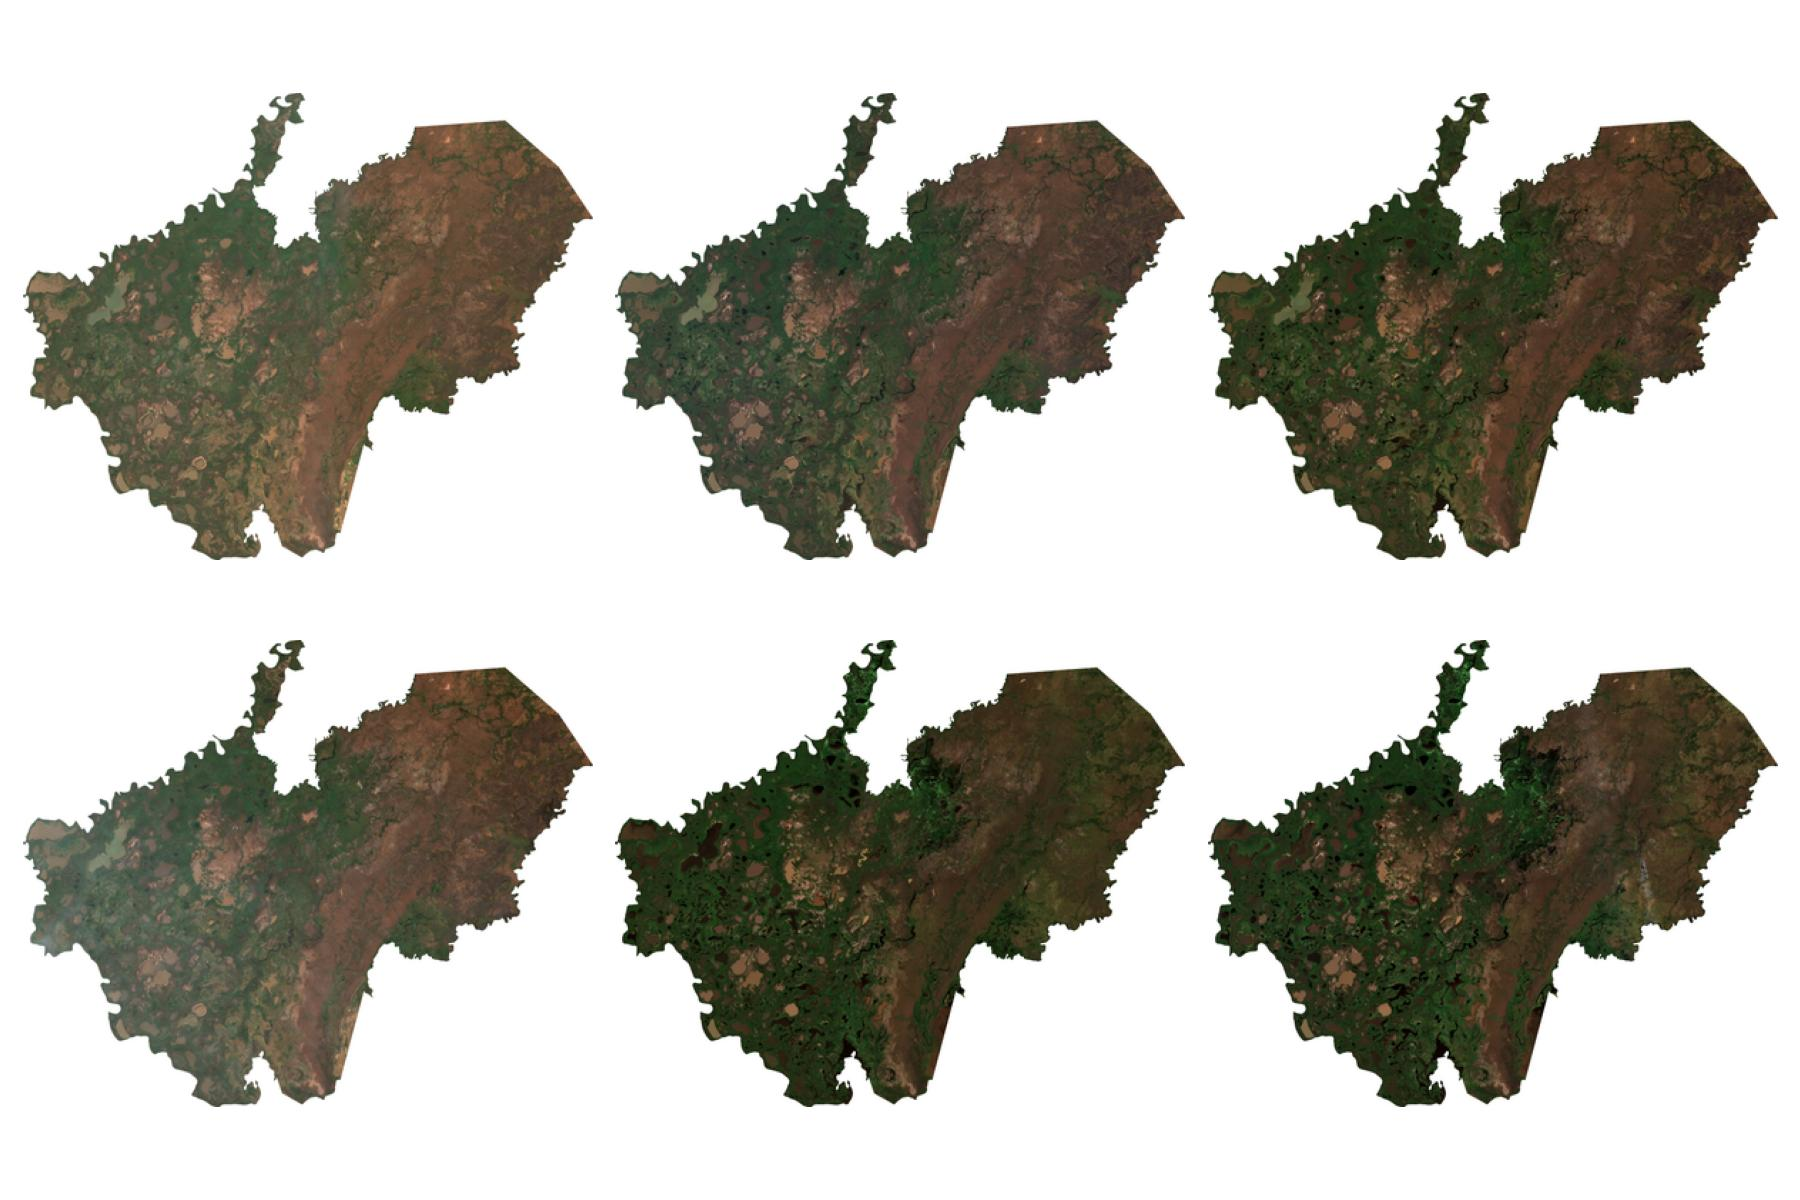
\includegraphics[width=0.65\textwidth]{./img/mosaic_mg_plot.jpg}
    \caption{Mosaicos selecionados pelo modelo CPLEX para a região de MT (PARNA do Pantanal), conforme listados na Tabela~\ref{tab:resultados_cplex}. A sequência apresenta sobreposição espacial mínima de 80\% e características radiométricas adequadas para análise multitemporal.}
    \label{fig:intersecoes}
\end{figure}

\vspace{-5mm}

A Tabela~\ref{tab:cobertura_comparacao} apresenta, para cada região, a cobertura real, o maior percentual de nuvens e o menor fator de qualidade entre os mosaicos selecionados pelo modelo CPLEX. Estes valores representam, respectivamente, os cenários mais desafiadores de cada região quanto à presença de nuvens e à qualidade radiométrica.

\vspace{-6mm}
\begin{table}[H]
    \centering
    \caption{Cobertura real, maior percentual de nuvens e menor fator de qualidade entre os mosaicos selecionados pelo modelo CPLEX para cada região.}
    \label{tab:cobertura_comparacao}
    \footnotesize
    \begin{adjustbox}{width=\textwidth}
    \begin{tabular}{llccc}
        \toprule
        \textbf{UF} & \textbf{UC} & \textbf{Cobertura (\%)} & \textbf{Nuvens (\%)} & \textbf{Fator Qualidade (\%)} \\
        \midrule
        BA      & PARNA Pau Brasil         & 100,00 & 18,44 & 74,65 \\
        AL      & APA Muricy               & 100,00 & 21,55 & 75,09 \\
        RS      & APA Ibirapuitã           & 98,93  & 3,36  & 73,08 \\
        MG-SP-RJ& PARNA Mantiqueira        & 89,14  & 1,86  & 94,33 \\
        PI-PE-CE& APA Chap.\ do Araripe    & 92,52  & 3,26  & 98,58 \\
        MT      & PARNA do Pantanal        & 100,00 & 0,00  & 99,90 \\
        \bottomrule
    \end{tabular}
    \end{adjustbox}
    \normalsize
\end{table}
\vspace{-5mm}

A análise detalhada mostra uma significativa redução nos mosaicos candidatos, com o modelo PLIM selecionando de 4 a 6 mosaicos por região, em contraste com o conjunto mais amplo sugerido pela heurística gulosa inicial. Esta otimização demonstra a eficácia do modelo em identificar os mosaicos com melhor relação entre cobertura útil e qualidade radiométrica para cada área de interesse, mantendo a sobreposição mínima de 80\% entre os mosaicos selecionados. Isto garante a consistência espacial necessária para análises temporais robustas.

Destaca-se a região PI-PE-CE, onde o modelo reduziu de 46 mosaicos candidatos para 6 (incluindo os mosaicos 9, 10, 11, 13, 31 e 33), e o PARNA Mantiqueira na região MG-SP-RJ, com redução de 45 para 6 mosaicos selecionados (incluindo os mosaicos 13-17 e 20). A BA apresentou o menor número de imagens por mosaico selecionado (apenas uma), enquanto PI-PE-CE teve três imagens em cada mosaico selecionado, o que reflete as diferentes complexidades geométricas e condições de imageamento das regiões.

A análise quantitativa demonstra que a metodologia alcançou excelentes resultados de áreas livres de nuvens nos mosaicos finais, com média superior a 98\% (considerando a ponderação por área), e variações conforme as condições climáticas regionais (de 98,93\% na APA Ibirapuitã a 78,45\% nas APAs de Alagoas). A Figura~\ref{fig:all_outputs} apresenta a visualização espacial de todos os mosaicos selecionados pelo modelo CPLEX para cada região. Esta visualização mostra como a abordagem proposta selecionou sequências de mosaicos que mantêm consistência espacial multitemporal, permitindo a análise multitemporal das áreas monitoradas.

Comparações diretas com trabalhos anteriores apresentam limitações metodológicas substanciais devido às diferenças fundamentais de objetivos: enquanto \citet{rodriguez-puerta:2024} concentraram-se exclusivamente na remoção de nuvens (atingindo $89,4\%$ de eficácia com CloudScore$^{+}$) e \citet{shepherd2020automated} priorizaram qualidade radiométrica em mosaicos sazonais de verão na Nova Zelândia (com nuvens residuais <0,1\%), a presente metodologia integra otimização multidimensional que contempla simultaneamente cobertura útil, qualidade radiométrica e sequências temporais consistentes, associando heurística gulosa com PLIM para garantir exclusividade de imagens e eficiência computacional em monitoramento contínuo de áreas geograficamente diversas.

\vspace{-2mm}
\begin{figure}[H]
    \centering
    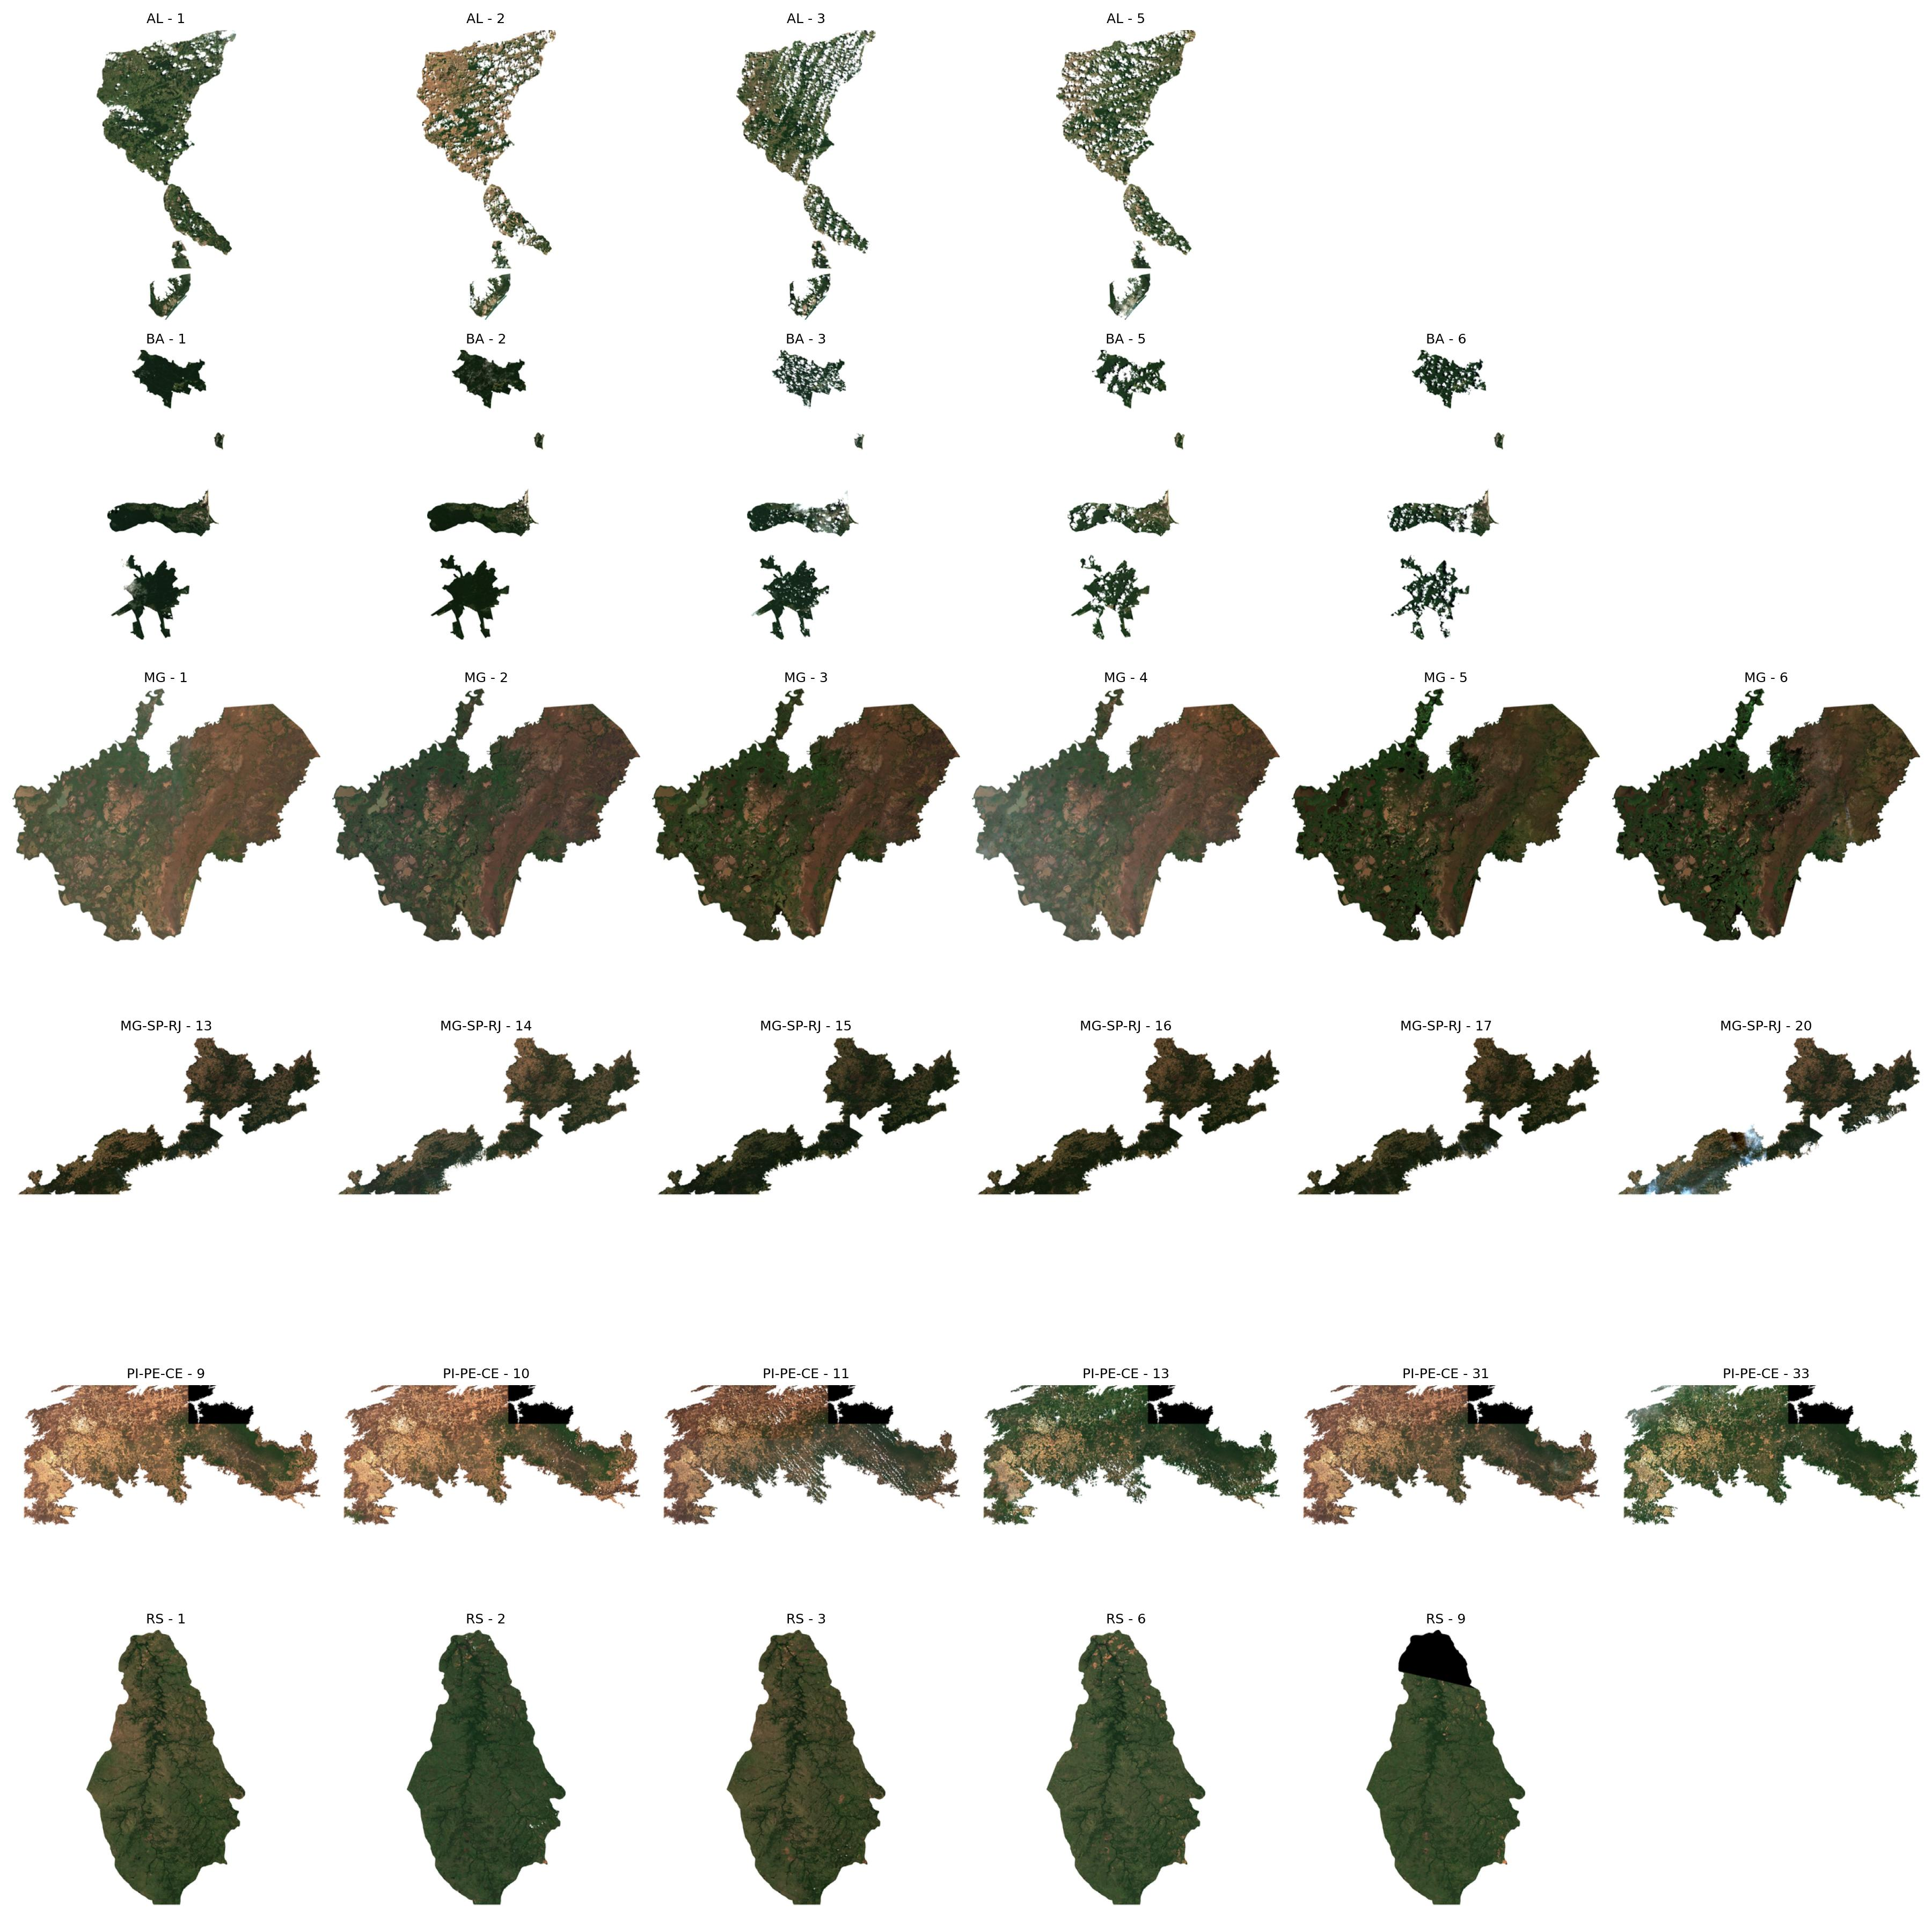
\includegraphics[width=0.65\textwidth]{img/all_selection.jpg}
    \caption{Visualização de todos os mosaicos selecionados pelo modelo CPLEX para cada região. As áreas aparecem reduzidas devido à sobreposição e escala, servindo apenas para referência geral da distribuição espacial das soluções.}
    \label{fig:all_outputs}
\end{figure}
\vspace{-2mm}

\vspace{-8mm}
\section{Conclusão}
\vspace{-4mm}
O trabalho atendeu ao objetivo de proporcionar uma solução eficiente para o monitoramento ambiental em Unidades de Conservação, permitindo a seleção de sequências de mosaicos que garantem cobertura útil, qualidade radiométrica e continuidade espacial multitemporal. Os mosaicos selecionados pelo modelo PLIM atingiram fatores de qualidade satisfatórios, com redução média de $96,2\%$ em relação à heurística gulosa inicial, selecionando entre 4 e 6 mosaicos por região. O controle da cobertura de nuvens foi eficaz, mantida abaixo de 10\% em cenários favoráveis como APA Ibirapuitã (3,36\%) e em níveis aceitáveis mesmo em regiões tradicionalmente nebulosas como a APA Muricy (21,55\%). A diversidade das UCs estudadas, de 3.708 ha a mais de 1 milhão de hectares, demonstra a aplicabilidade da metodologia em diferentes contextos geográficos e climáticos.

A abordagem híbrida desenvolvida, com suas etapas distintas --- heurística gulosa (Fase 1) e otimização PLIM (Fase 2) --- mostrou-se efetiva para obter soluções de qualidade. O algoritmo PLIM garante que os mosaicos selecionados mantenham sobreposição espacial de pelo menos 80\%, permitindo análises multitemporais consistentes sobre as mesmas regiões.

A incorporação de penalizações específicas para cobertura de nuvens na função objetivo do modelo PLIM resultou em soluções otimizadas, com 202 imagens selecionadas no total. Mesmo nas áreas com maior complexidade geométrica, como a APA Chapada do Araripe e o PARNA Mantiqueira, o método alcançou coberturas satisfatórias de 92,52\% e 89,14\%, respectivamente.

Embora o método assegure intervalos curtos entre imagens de um mesmo mosaico, o espaçamento entre mosaicos consecutivos pode variar devido às condições climáticas, refletindo limitações inerentes ao sensoriamento óptico.

Trabalhos futuros podem explorar recortes parciais e janelas temporais maiores para cobrir lacunas em áreas com alta nebulosidade, além de incorporar imagens SAR na função objetivo. Pretende-se também expandir a aplicação para diferentes regiões e perfis climáticos, e investigar estratégias de fusão de imagens para manter a visualização global em períodos de disponibilidade limitada.
\vspace{-6mm}
\begingroup
  \sloppy
  \emergencystretch=1em
  \bibliographystyle{sbpo}
  \bibliography{references}
  \nocite{*}
\endgroup
\end{document}